\section{アンカーの発話群検出実験}
\label{chapter:get_anchor}
\subsection{実験方法}
同一話者の可能性が高い発話区間を結合、i-vectorを再抽出してアンカーの発話区間検出を行った。発話区間の結合手法は以下の通りである。

\begin{itemize}
\item 手法1 : 発話の間隔情報を考慮した発話区間の結合手法
\item 手法2 : 発話環境を考慮した発話区間の結合手法
\item 手法3 : 手法1 + 手法2
\end{itemize}

前後の発話区間を結合する際にi-vectorのコサイン類似度を用いるが、同一話者間の発話であっても発話の長さによってとりうるコサイン類似度が大きく異なる。そのため、発話の長さによって結合するか否かのコサイン類似度の閾値を変更する必要がある。これは、図\ref{fig:time_cos}を用いて決定した。

\begin{figure}[H]
  \begin{center}
    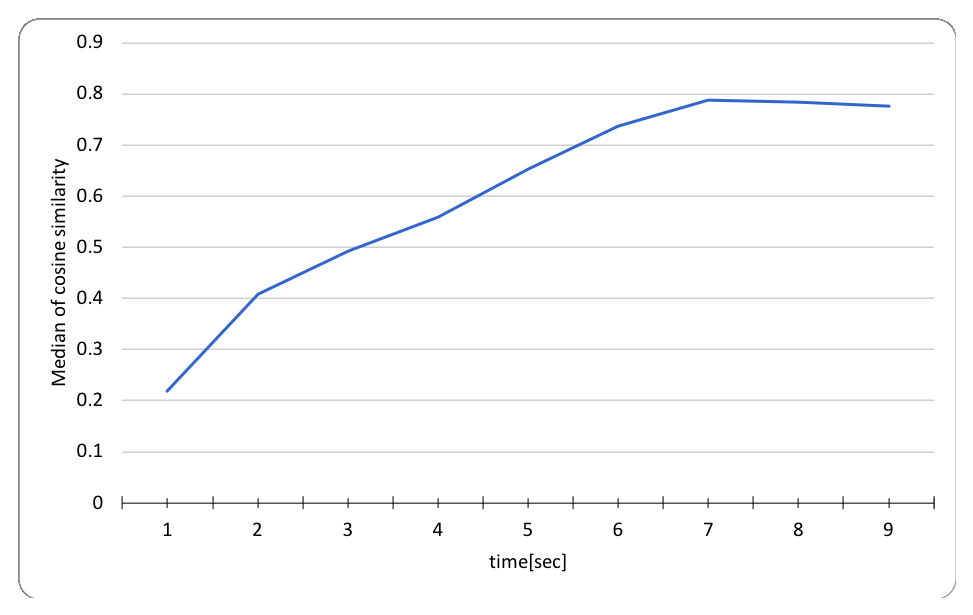
\includegraphics[scale=0.8]{./figure/time_cos.eps}
  \end{center}
  \caption{発話の長さに対するコサイン類似度の平均 \label{fig:time_cos}}
\end{figure}

発話長が2秒以下までは発話長が長くなるごとに急激にコサイン類似度が上昇している。次に、発話長が7秒までのとき、なだらかにコサイン類似度が上昇している。発話長が7秒以上になるとコサイン類似度は停滞する。以上のことから、発話の長さを$T$[sec]としたとき、決定した閾値を表\ref{table:decide_thcos}に示す。

\begin{table}[H]
  \begin{center}
    \caption{結合の閾値 \label{table:decide_thcos}}
    \begin{tabular}{|c||c|} \hline
時間条件 & コサイン類似度の閾値  \\ \hline
$T <$ 2 &  0.1 \\ \hline
2 $\leqq T <$ 7 &  0.3  \\ \hline
7 $< T$ &  0.7 \\ \hline
    \end{tabular}
  \end{center}
\end{table}

また、手法1では非発話区間の長さの閾値$T_{time}$によって結合するか否かを決定するため、閾値$Th_{time}$によって発話区間の結合精度が変化する。本実験では図\ref{fig:same_sp}より、$Th_{time}$を0.8秒から1.5秒までを0.1秒刻みで行なった。

i-vectorを用いたアンカーの発話区間抽出は\ref{section:clustering}節の手法を用いる。i-vectorの抽出には、ALIZEとLIR RALを用いる。i-vectorの抽出に使用するUBMモデルの学習には読み上げ音声\cite{ATR}を使用する。読み上げ音声に収録されている各発話データからi-vectorを抽出する。発話データから抽出する音響特徴パラメータを表\ref{iv_feature2}に示す。また混合数は32とした。$Th_{cos}$は0.8から1.5までの範囲を0.1刻みで検証を行う。また、Baselineとしてi-vectorの再抽出を行わずにアンカーの発話区間検出を行う。\par

\begin{table}[H]
  \begin{center}
    \caption{使用する音響特徴パラメータ \label{iv_feature2}}
    \begin{tabular}{|c||c|} \hline
      特徴量 & 次元数\\ \hline
      MFCC & 19  \\ 
      POW & 1  \\ 
      $\Delta$MFCC & 19 \\ 
      $\Delta$POW & 1 \\ 
      $\Delta\Delta$MFCC & 19 \\ 
      $\Delta\Delta$POW & 1 \\ \hline
      計 & 60 \\ \hline
    \end{tabular}
  \end{center}
\end{table}

\subsection{評価方法}
評価は、検出されたアンカーの発話区間と正解ラベルを比較して行う。

\begin{table}[H]
\begin{center}
    \caption{アンカーの発話区間の正誤判定 \label{table:clustering}}
\begin{tabular}{|c|c|c|c|l}
\cline{1-4}
\multicolumn{2}{|c|}{\multirow{2}{*}{}} & \multicolumn{2}{c|}{「発話者」のラベルが付与された発話区間} &  \\ \cline{3-4}
\multicolumn{2}{|c|}{}                  & アンカーの発話区間        & アンカー以外の発話区間        &  \\ \cline{1-4}
\multirow{2}{*}{判定結果}        & 正        & $TP$                  & $FP$                   &  \\ \cline{2-4}
& 誤        & $FN$                  & $TN$                   &  \\ \cline{1-4}
\end{tabular}
\end{center}
\end{table}

表\ref{table:clustering}を用いて、$P$(適合率(Precision))と$R$(再現率(Recall))を式\ref{calc:precision2}と式\ref{calc:recall2}のようにそれぞれ定義する。また、$F$値($F-measure$)を式\ref{calc:fmeasure2}のように定義する。

\begin{equation}
\label{calc:precision2}
P = \frac{TP}{TP + FP}
\end{equation}

\begin{equation}
\label{calc:recall2}
R = \frac{TP}{TP + FN}
\end{equation}

\begin{equation}
\label{calc:fmeasure2}
F = \frac{1}{\frac{1}{P} + \frac{1}{R}}
\end{equation}

ここで$P$と$R$はそれぞれ適合率、再現率を表す。

また、検出したアンカーの発話区間の割合を式\ref{calc:anchor_acc}のように定義して評価する。

\begin{equation}
\label{calc:anchor_acc}
Acc_{time} = \frac{検出したアンカーの発話区間の時間数}{アンカーの発話区間の時間数}
\end{equation}

本実験では、評価方法として適合率、再現率、$F$値、$Acc_{time}$を用いる。

\subsection{実験結果}
アンカーの発話区間検出精度を以下に示す。本節では各手法で最も良いF値を示した条件の結果を記載している。その他の条件の結果は付録で記載する。

\begin{figure}[H]
  \begin{center}
    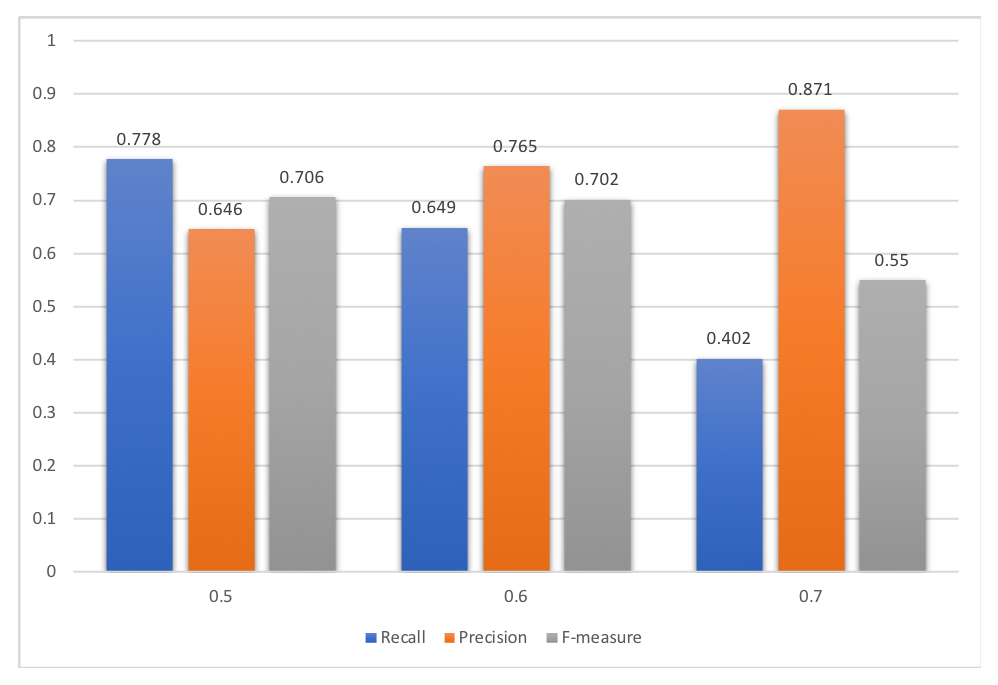
\includegraphics[scale=0.8]{./figure/get_anchor_baseline.eps}
  \end{center}
  \caption{アンカーの発話区間検出精度のBaseline \label{fig:result_anchor_baseline}}
\end{figure}

\begin{figure}[H]
  \begin{center}
    \includegraphics[scale=0.8]{./figure/get_anchor_prob1.eps}
  \end{center}
  \caption{提案手法1によるアンカーの発話区間検出精度 ($Th_{time}=1.0$) \label{fig:result_anchor_prob1}}
\end{figure}

\begin{figure}[H]
  \begin{center}
    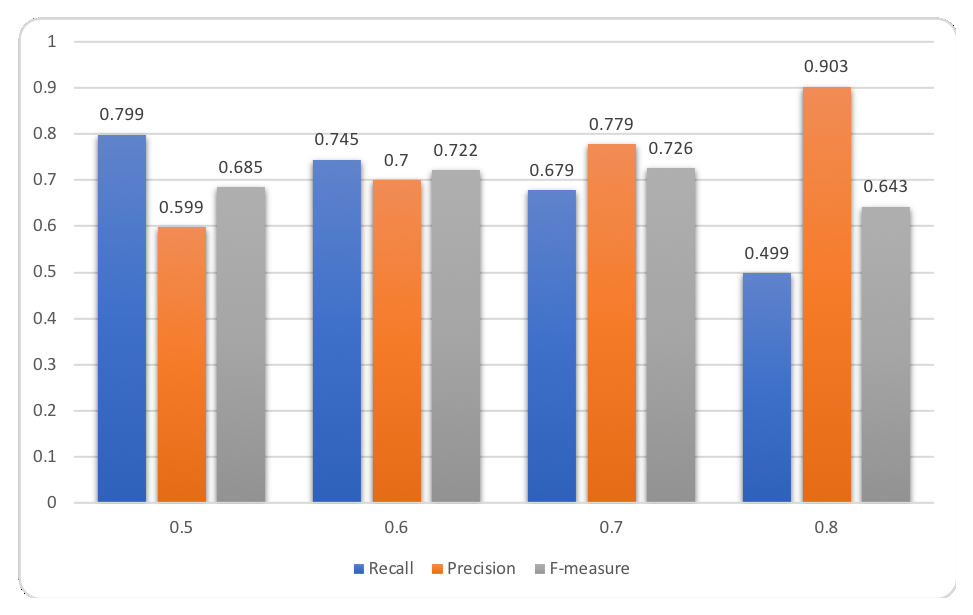
\includegraphics[scale=0.8]{./figure/get_anchor_prob2.eps}
  \end{center}
  \caption{提案手法2によるアンカーの発話区間検出精度 \label{fig:result_anchor_prob2}}
\end{figure}

\begin{figure}[H]
  \begin{center}
    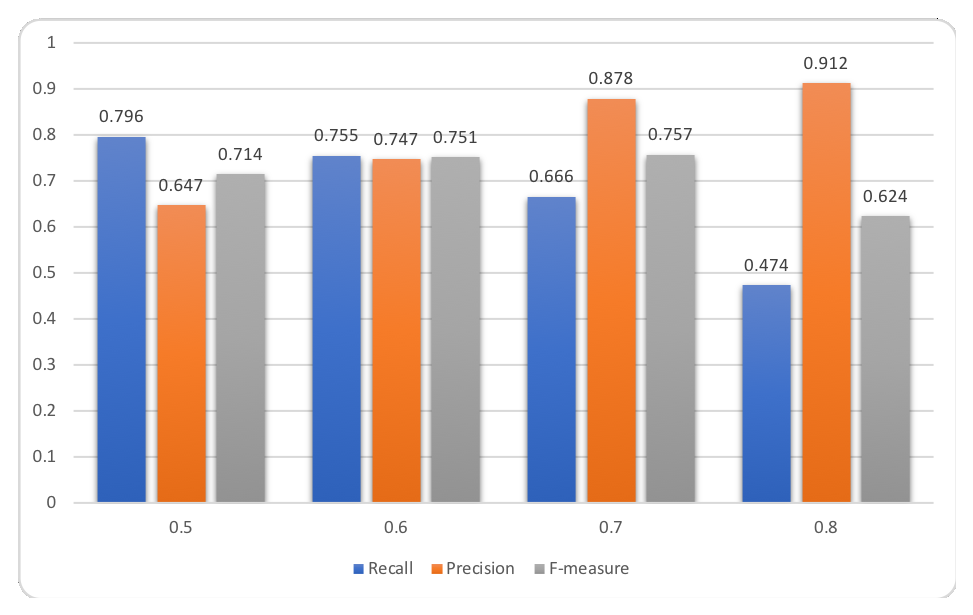
\includegraphics[scale=0.8]{./figure/get_anchor_prob3.eps}
  \end{center}
  \caption{提案手法3によるアンカーの発話区間検出精度 ($Th_{time}=1.2$) \label{fig:result_anchor_prob3}}
\end{figure}

実験の結果、発話区間を結合して再抽出したi-vectorを用いた手法が全体的に高い精度を示した。Baselineは$Th_{cos}$が0.8のときクラスタが小さくなりすぎたためアンカーの発話区間を検出出来なかった。また、Baselineは$Th_{cos}$が0.5のときがF-measureが最も高い値をとるのに対して、本提案手法では$Th_{cos}$が0.7のとき、F-measureが最も高い値をとった。\par
本実験の提案手法では、手法1が最も発話区間検出精度が高く、F値が0.795であった。また、いずれの手法においても$Th_{cos}$が小さい時にはRecallが高く、大きい時にはPrecisionが高くなる傾向が確認された。

\subsection{考察}
Baselineと再抽出したi-vectorを用いた各提案手法を比較したとき、再抽出したi-vectorを用いた手法の方が$Th_{cos}$を高くした時に発話区間検出精度が向上している。このことから、i-vectorの抽出精度が向上したと考えられる。\par

